\chapter{Kinetic Data Structures Framework}
\label{chapter-kds}
\ccChapterAuthor{Daniel Russel}
\minitoc



%\def\c#1{\protect{\em{\small #1}}}


%\def\KK{\ccc{KineticKernel}}
%\def\MOT{\ccc{MovingObjectTable}}
%\def\S{\ccc{Solver}}
%\def\Sim{\ccc{Simulator}}
%\def\IK{\ccc{InstantaneousKernel}}
%\def\MF{\ccc{MotionFunction}}
%\def\SK{\ccc{StaticKernel}}
%\def\Int{\ccc{Interval_NT}}
%\def\FG{\ccc{FunctionGenerator}}
%\def\R{\ccc{Root}}
%\def\P{\ccc{Function}}
%\def\PK{\ccc{FunctionKernel}}
%\def\RK{\ccc{RootKernel}}
%\def\KP{\ccc{KineticPredicate}}
%\def\CF{\ccc{ConstructedFunction}}
%\def\Sk{\ccc{Sort}}

\def\note#1{$\langle\langle${\bf #1}$\rangle\rangle$}
%\message{Remove note before final version!}
%\def{\th}{^{\rm th}}

% space tweaks
%\addtolength{\parskip}{-1pt}

\section{Todo}

\subsection{General thoughts}

\begin{itemize}

\item I like the idea of changing MovingObjectTable to ActiveObjectTable. Not sure if Notifying\_table should follow suit. 

\item Regular triangulation 3 is not entirely working.

\item I reorganized out of existance my 3D demos.

\item The other trajectory modification events need to be documented

\item There is no testing of the Delaunay 3 Visitor class. 

\item The architeture figure goes to the end for some reason. 

\end{itemize}

%%% Local Variables: 
%%% mode: latex
%%% TeX-master: t
%%% End: 



This chapter describes a framework for implementing kinetic data
structures and sweepline algorithms as well as several kinetic data
structures implemented on top of this framework. We first, in
Section~\ref{sec:kds_intro} introduce kinetic data structures and
sweepline algorithms. We then present kinetic datastructures for
Delaunay triangulations in two and three dimensions in
Section~\ref{sec:provided_kdss}. Following that, in
Section~\ref{sec:architecture} we discuss the architecture of the
framework and finally we give several examples of using the framework
in Section~\ref{sec:examples}. The framework makes heavy use of our
\ccc{Polynomial} package to provide models of the \ccc{FunctionKernel}
concept.

%%%%%%%%%%%%%%%%%%%%%%%%%%%%%%%%%%%%%%%%%%%%%%%%%%%%%%%%%%%%%%%%%%%%
\section{Kinetic Data Structures and Sweep Algorithms}
\label{sec:kds_intro}
%%%%%%%%%%%%%%%%%%%%%%%%%%%%%%%%%%%%%%%%%%%%%%%%%%%%%%%%%%%%%%%%%%%%


\subsection{Kinetic Data Structures}
Motion is ubiquitous in the world around us and is a feature of many
problems of interest to computational geometers. Kinetic data
structures were introduced by Basch et. al. in '97~\cite{basch97data,
guibas98kinetic}. They exploit the combinatorial nature of most
geometric data structures---the combinatorial structure remains
invariant under some motions of the underlying geometric primitives
and, when the structure does need to change, it does so at discrete
times and in a limited manner. Algorithms that fit within the kinetic
data structures framework have been found for a number of geometric
constructs of interest, including Delaunay and regular triangulations
in two and three dimensions (implementations of which are provided)
and various types of clustering.

Computational geometry is built on the idea of
\textit{predicates}---functions of the description of geometric
primitives which return a discrete set of values. Many of the
predicates reduce to determining the sign of an algebraic expression
of the representation (i.e.\ coordinates of points) of the geometric
primitives. For example, to test whether a point lies above or below a
plane, we compute the dot product of the point with the normal of the
plane and subtract the plane's offset along the normal. If the result
is positive, the point is above the plane, zero on the plane, negative
below.

The validity of many combinatorial structures built on top of
geometric primitives can be proved by checking a finite number of
predicates of the primitives. These predicates are called {\em
  certificates}. For example, a three-dimensional convex hull is
proved to be correct by checking, for each face, that all points are
below the outward facing plane supporting it.

The kinetic data structures framework is built on top of this view of
computational geometry. Let the geometric primitives move by replacing
each of their coordinates with a function of time. As time advances,
the primitives now trace paths in space called {\em trajectories}. The
values of the certificates which proved the correctness of the static
structure now become functions of time, called the {\em certificate
  functions}. As long as these functions have the correct value, the
original structure is still correct. However, if one of the
certificate functions changes value, the original structure must be
updated and some new set of certificate functions computed. We call
such occurrences {\em events}.

Maintaining a kinetic data structure is then a matter of determining
which certificate function changes value next (typically this amounts
to determining which certificate function has the first root after the
current time) and then updating the structure and certificate
functions.

The {\em Kinetic data structures framework} provides a basis for
implementing such data structures on moving data and allows the user
to easily change between exact, filtered or numeric computation.

\subsection{Sweepline view}

Instead of sweeping over time, we can instead sweep over one of the
geometric coordinates. For example, we can compute a planar
arrangement of x-monotone curves by sweeping along the x-coordinate
from negative infinity to infinity, tracking the order the vertical
order of the curves. The certificates are then that one curve is above
another at the current ``time'' or x value. Each time two curves
intersect, we must exchange their vertical order. The computation
entailed is exactly the same as tracking the sorted order of a set of
points as they move along the real line.

\section{Using Kinetic Data Structures\label{sec:kds_provided_kdss}}


There are five provided kinetic data structures. They are
\begin{description}
\item[\ccc{Kinetic::Sort<Traits, Visitor>}] maintain a list of points
sorted by x-coordinate.
\item[\ccc{Kinetic::Delaunay_triangulation_2<Traits, Visitor,
    Triangulation>}] maintain the Delaunay triangulation of a set of
  two dimensional points
\item[\ccc{Kinetic::Delaunay_triangulation_3<Traits,Visitor,
    Triangulation>}] maintain the Delaunay triangulation of a set of
  three dimensional points.
\item[\ccc{Kinetic::Regular_triangulation_3<Traits, Visitor,
Triangulation>}] maintain the regular triangulation of a set of waiting
three dimensional points.
\item[\ccc{Kinetic::Enclosing_box_2<Traits>},
  \ccc{Kinetic::Enclosing_box_3<Traits>}] restrict points to stay
  within a box by bouncing them off the walls.
\end{description}


\subsection{Two Dimensional Delaunay}
\label{sec:sort_example}

Using a kinetic data structure can be as simple as the following:
\label{fig:sort_program}
\ccIncludeExampleCode{Kinetic_data_structures/sort.C}

In the example, first the Kinetic::SimulationTraits object is chosen
(in this case one that supports exact computations). Then the kinetic
data structure is defined, using the chosen traits object and a
visitor class which logs changes to the sorted list.  Next, instances
of the two are created and a set of points is read from a file. Then,
the simulator is instructed to process all the events until the end of
the simulation.  Finally, a record of what happened is printed to the
terminal.

Several important things happen behind the scenes in this example.
First, the Kinetic::ActiveObjectsTable which holds the moving points
notifies the kinetic data structure that new points have been added to
the simulation. Second, the \ccc{Kinetic::Sort<Traits,Visitor>} kinetic data structure
registers its events with the Kinetic::Simulator by providing a time
and a proxy object. When a particular event occurs, the
Kinetic::Simulator calls a function on the proxy object which in turn
updates the kinetic data structure.

The example illustrates how to monitor the supplied data structures as
they evolve by using a Kinetic::SortVisitor object---a small class whose
methods are called whenever the kinetic data structure changes. Hooks
for such visitor concepts are provided for all of the shipped kinetic
data structures. In the case of kinetic sorting, the visitor's
methods are called every time a new point is inserted in the sorted
list, when one is removed, or when two points are swapped in the
sorted order. 


The visitor concept is quite powerful, allowing us, for example, to
implement a data structure for computing and storing two-dimensional
arrangements of $x$-monotone curves on top of the
\ccc{Kinetic::Sort<Traits, Visitor>} data structure using about 60
lines of code. This sweepline code is presented in
Section~\ref{sec:sweepline_example}.




\subsection{Visualization of Kinetic Data Structures\label{sec:kds_delaunay_2_example}}


The framework includes Qt widgets for displaying kinetic data
structures in two and three dimensions. The following example shows
using the two dimensional widget with a Delaunay triangulation:

\begin{ccExampleCode}
#include <CGAL/Kinetic/Exact_simulation_traits.h>
#include <CGAL/Kinetic/Delaunay_triangulation_2.h>
#include <CGAL/Kinetic/Enclosing_box_2.h>
#include <CGAL/Kinetic/IO/Qt_moving_points_2.h>
#include <CGAL/Kinetic/IO/Qt_triangulation_2.h>
#include <CGAL/Kinetic/IO/Qt_widget_2.h>

int main(int argc, char *argv[]) {
    using namespace CGAL::Kinetic;
    typedef Exact_simulation_traits Traits;
    typedef Delaunay_triangulation_2<Traits> Del_2;
    typedef Enclosing_box_2<Traits> Box_2;
    typedef Qt_widget_2<Traits::Simulator> Qt_widget;
    typedef Qt_moving_points_2<Traits, Qt_gui> Qt_mps;
    typedef Qt_triangulation_2<Del_2, Qt_widget, Qt_mps> Qt_dt2;
    
    // create a simulation traits and add two KDSs:
    // a kinetic Delaunay triangulation and an enclosing box;
    // the moving points bounce against the walls of the enclosing box
    Traits tr;
    Box_2::Handle box = new Box_2(tr);
    Del_2::Handle kdel = new Del_2(tr);

    // register the simulator, set of moving points and
    // Delaunay triangulation with the kinetic Qt widget
    Qt_widget::Handle qt_w = new Qt_widget(argc, argv, tr.simulator_handle());
    Qt_mps::Handle qt_mps = new Qt_mps(qt_w, tr);
    Qt_dt2::Handle qt_dt2 = new Qt_dt2(kdel, qt_w, qt_mps);

    // read the trajectories of the moving points
    //  the simulation traits automatically inserts them in the two KDSs
    // and schedules the appropriate kinetic events; as in the kinetic
    // sorting example this is done with appropriate notifications
    std::ifstream in("data/points_2");    
    in  >> *tr.active_points_2_table_handle();

    // run the interactive kinetic simulation
    return qt_w->begin_event_loop();
};
\end{ccExampleCode}

The example shows how to use a number of additional features of the
framework. First, it shows that two kinetic data structures
(\ccc{Kinetic::Delaunay_triangulation_2<Traits, Triangulation>} and
\ccc{Kinetic::Enclosing_box_2<Traits>}) can coexist on the same set of
points without any extra effort. Both interact with the moving points
through the active objects table, and never need to directly interact
with one another. Second, objects (like
\texttt{qt\_w}, \texttt{qt\_mps} and \texttt{qt\_dt2}) are all stored
by using reference counted handles (\texttt{Object::Handle}). This
allows them to share references to one another without the user having
to worry about memory management and order of deletion.  For example,
the \ccc{Kinetic::Qt_triangulation_2<KineticDelaunay_2, QtWidget_2,
Qt_moving_points_2>} object needs a handle to the kinetic
triangulation, in order to get the structure to display, and a handle
to the \ccc{Active_points_1_table} to get the coordinates of the
points.


Finally, the example shows how to use the graphical interface elements
provided, see Figure~\ref{fig:kds_qtwidget_capture}. Our package includes
\texttt{Qt} widgets for displaying kinetic geometry in two and three
dimensions. In addition to being able to play and pause the
simulation, the user can step through events one at a time and reverse
the simulation to retrace what had happened. The three-dimensional
visualization support is based on the Coin library http://www.coin3d.org.

\begin{figure*}[htb]
\begin{ccTexOnly}
\begin{center}
1.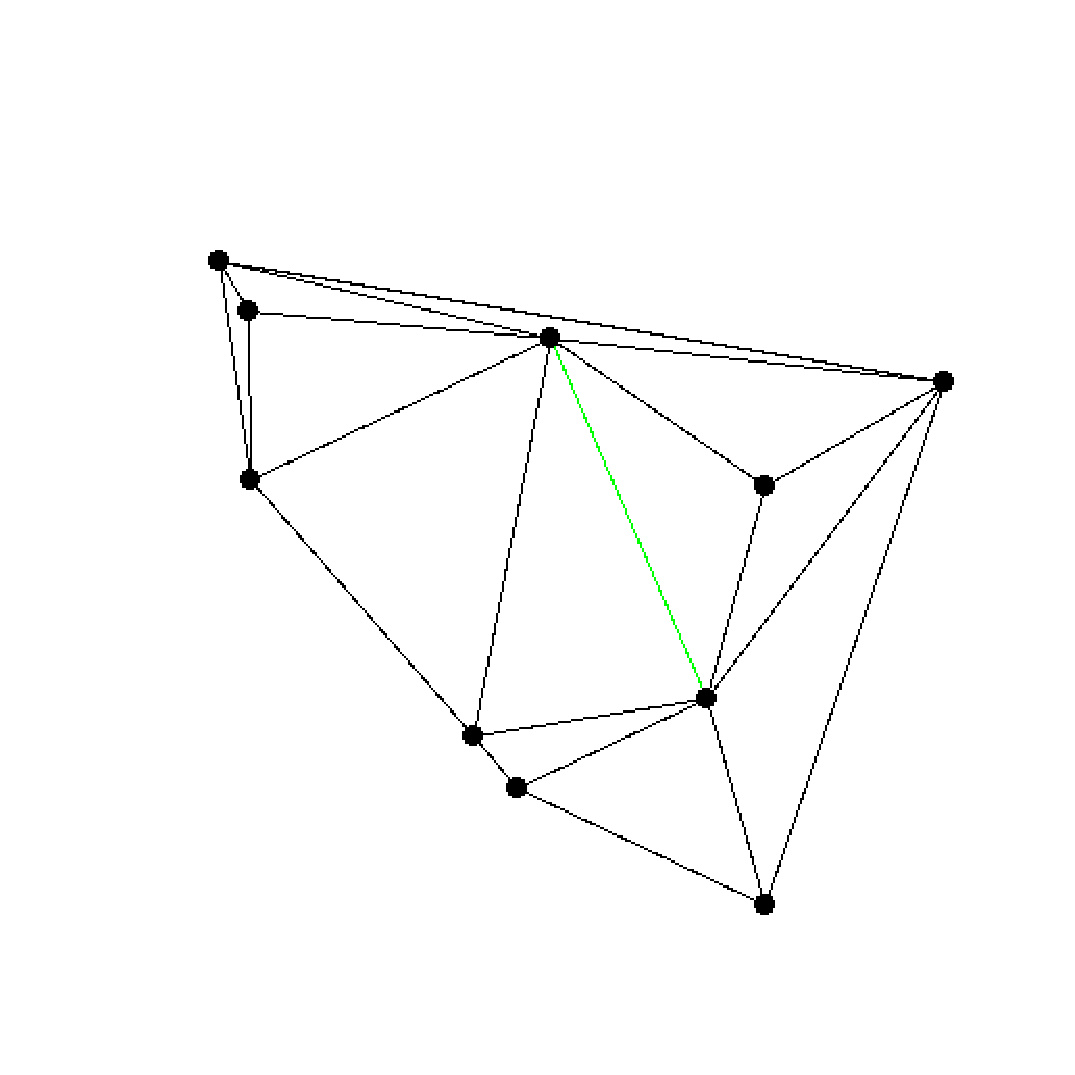
\includegraphics[ scale=.2]{Kinetic_data_structures/delaunay_0} 
2.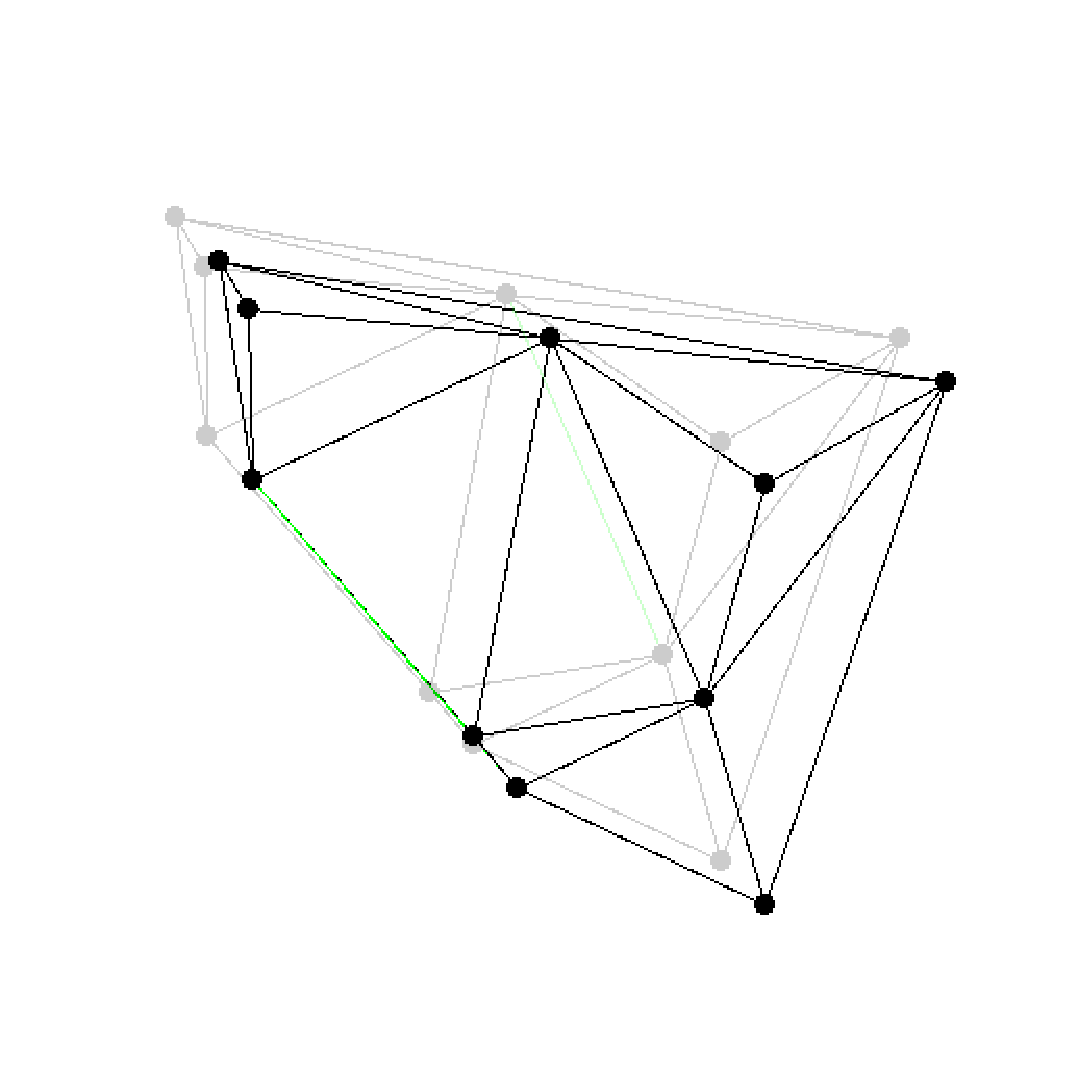
\includegraphics[ scale=.2]{Kinetic_data_structures/delaunay_1}
3.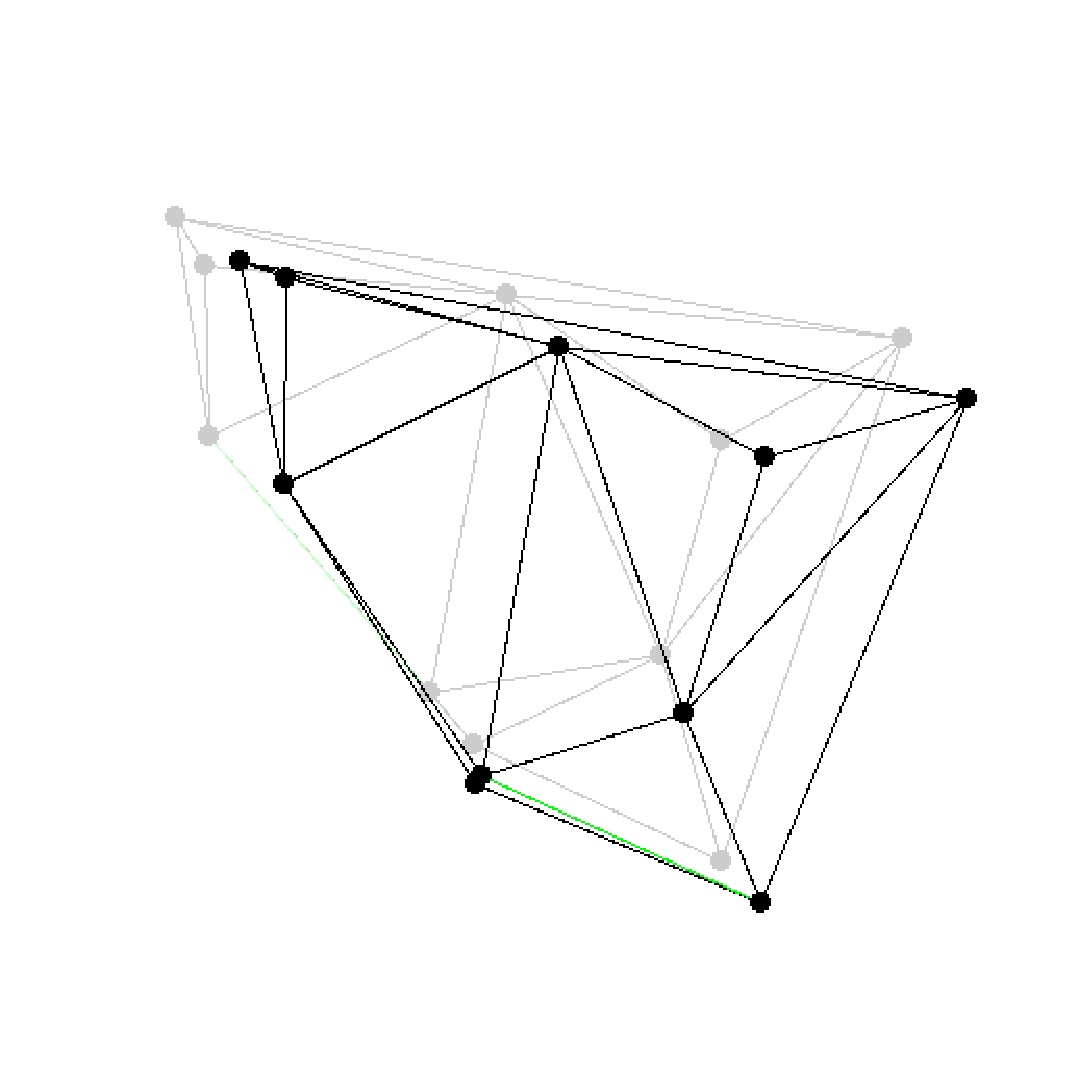
\includegraphics[ scale=.2]{Kinetic_data_structures/delaunay_2}\\
4.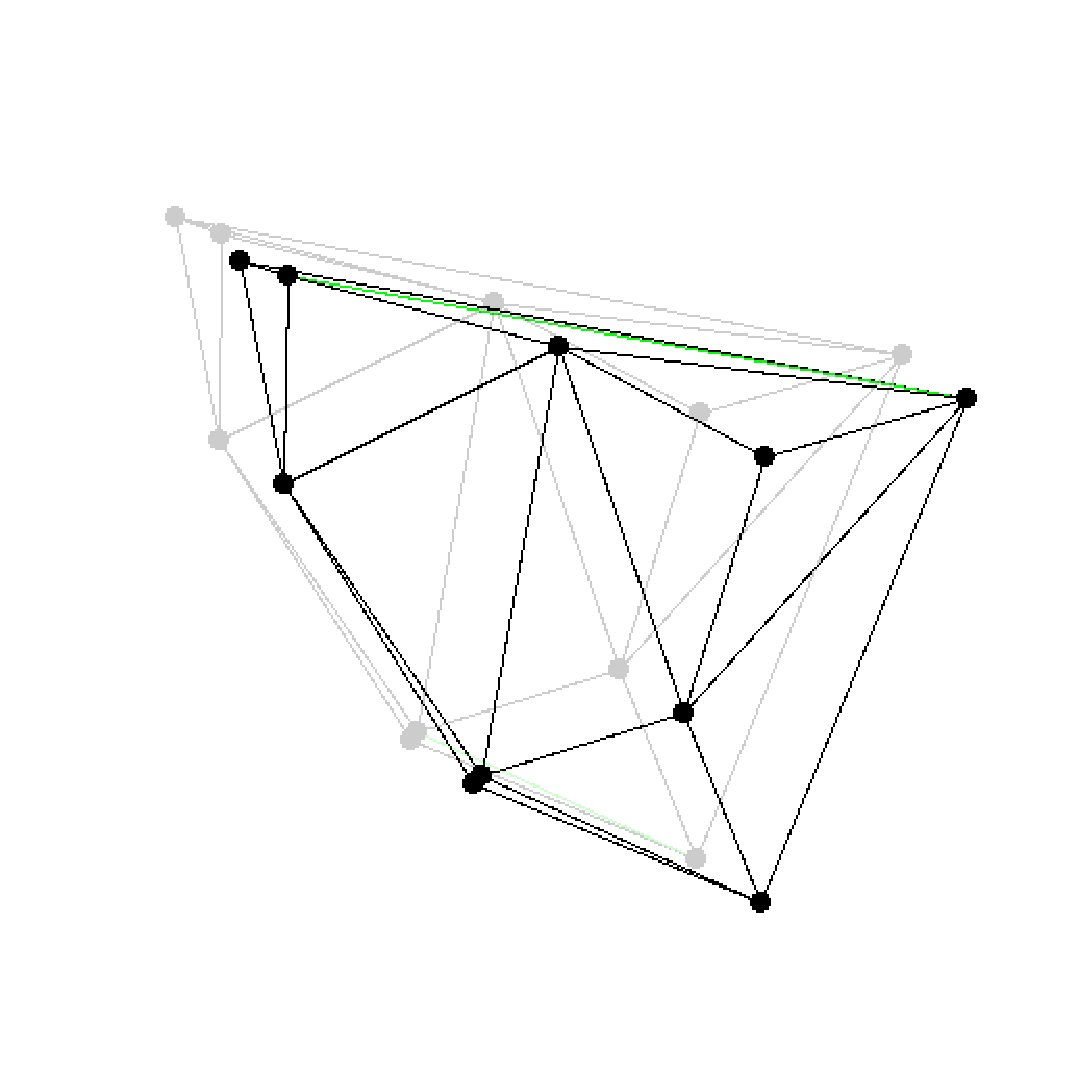
\includegraphics[ scale=.2]{Kinetic_data_structures/delaunay_3}
5.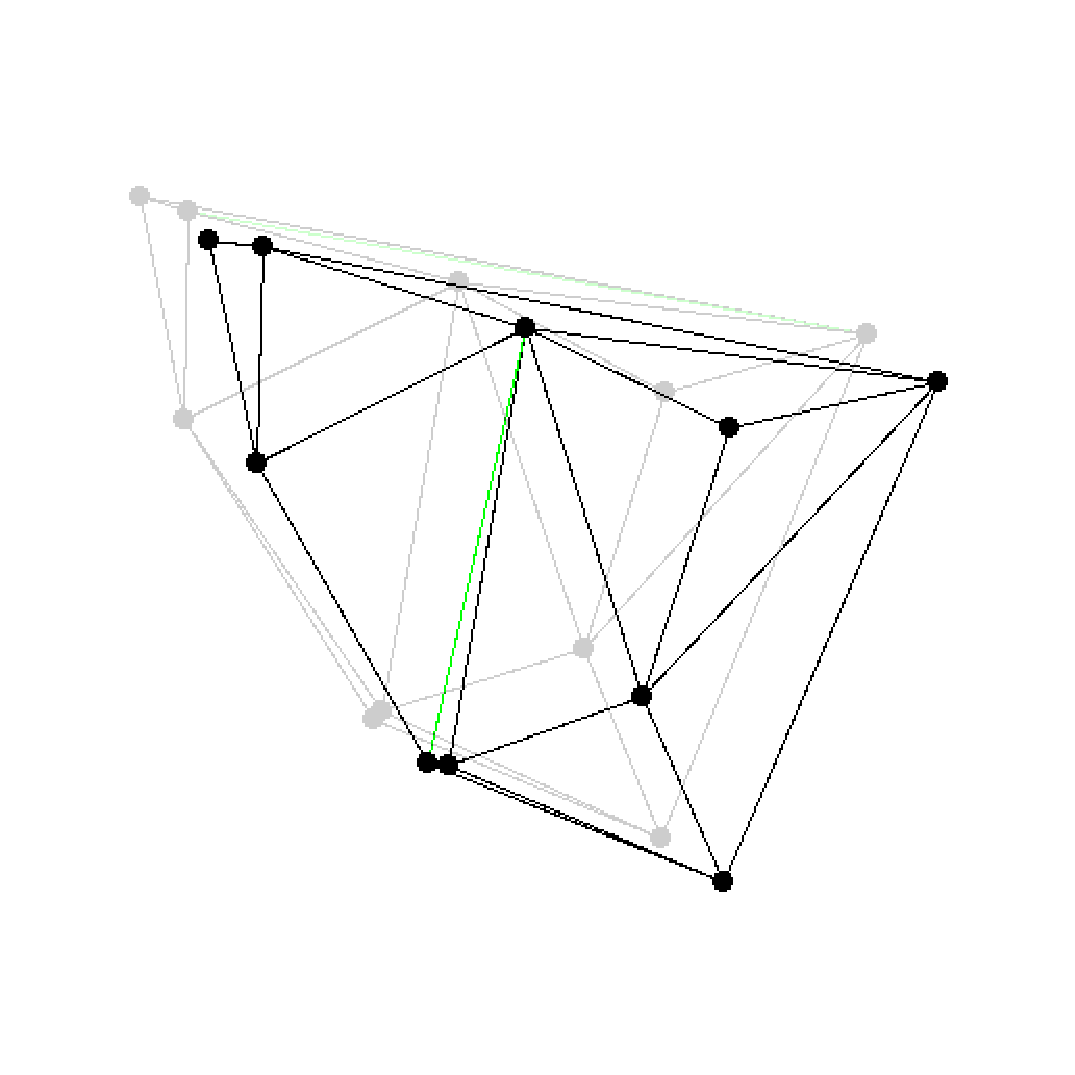
\includegraphics[ scale=.2]{Kinetic_data_structures/delaunay_4}
6.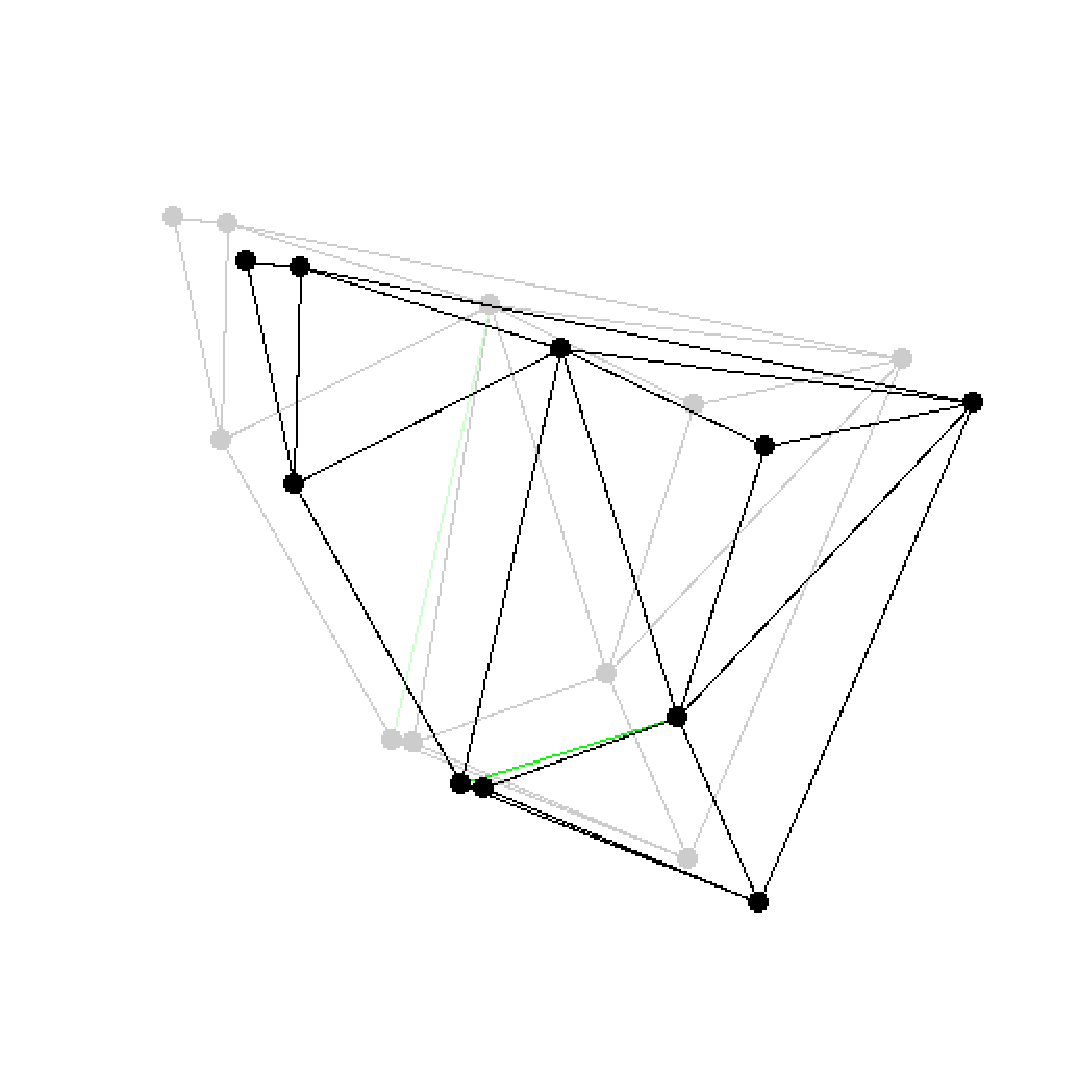
\includegraphics[ scale=.2]{Kinetic_data_structures/delaunay_5}\\
7.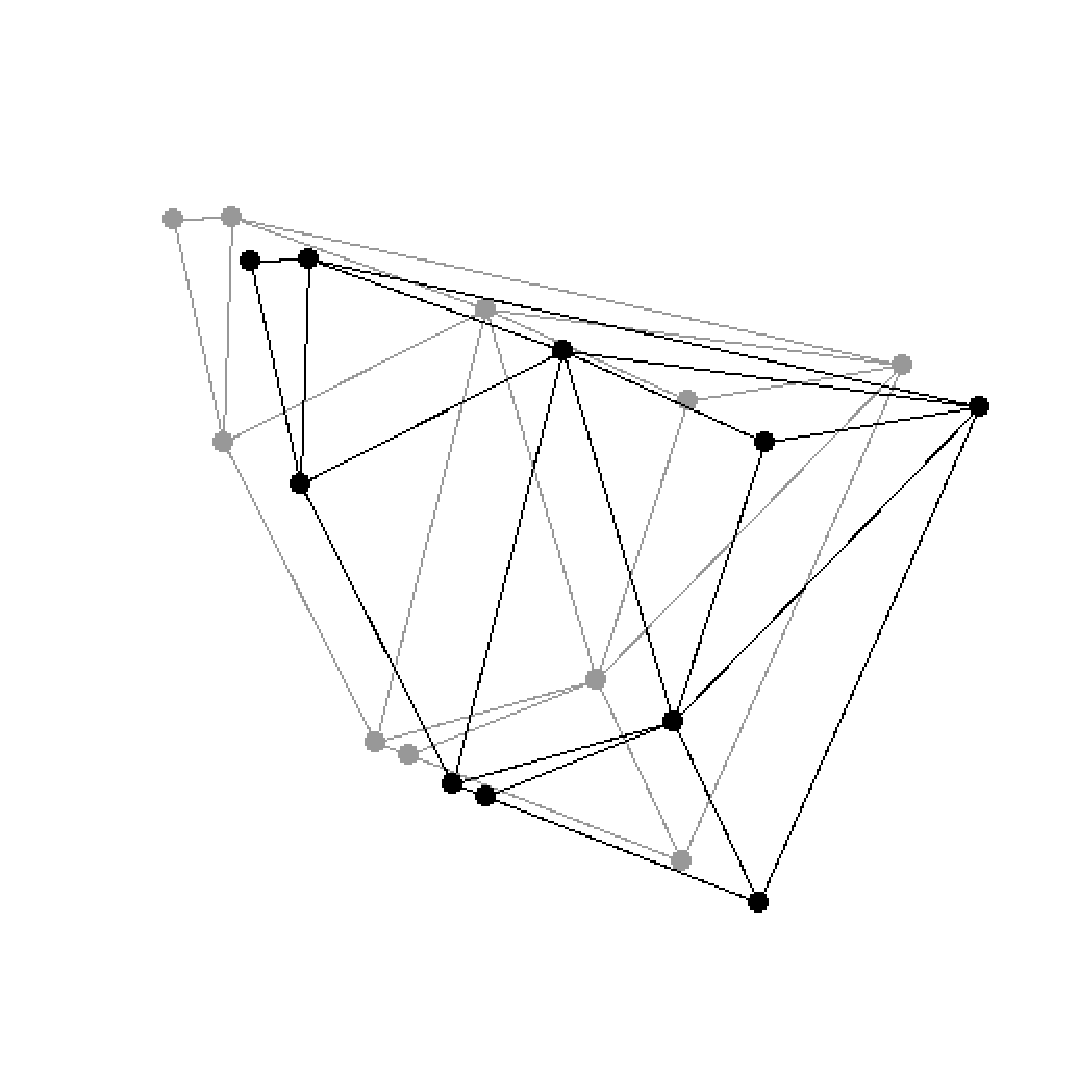
\includegraphics[ scale=.2]{Kinetic_data_structures/delaunay_6}
8.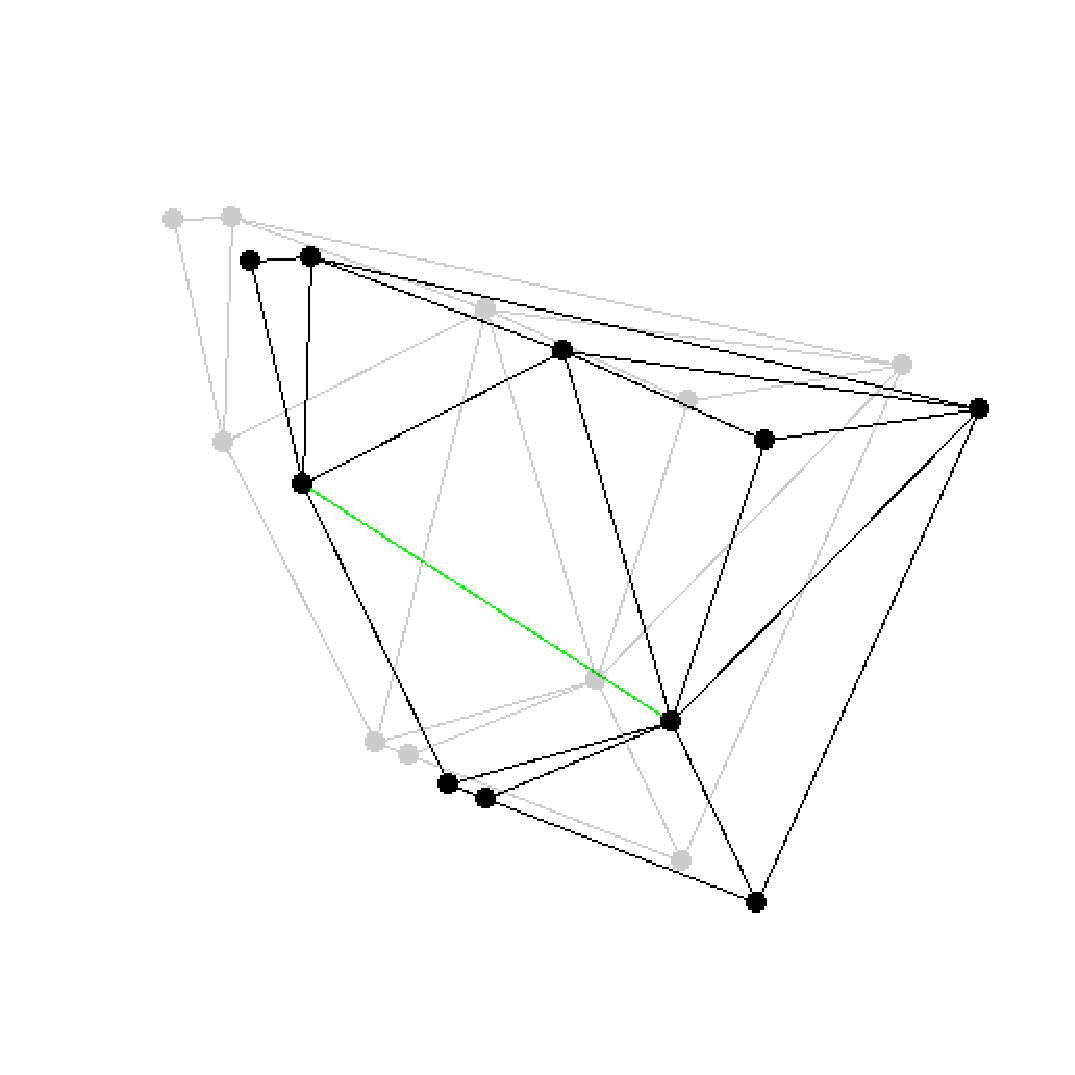
\includegraphics[ scale=.2]{Kinetic_data_structures/delaunay_7}
9.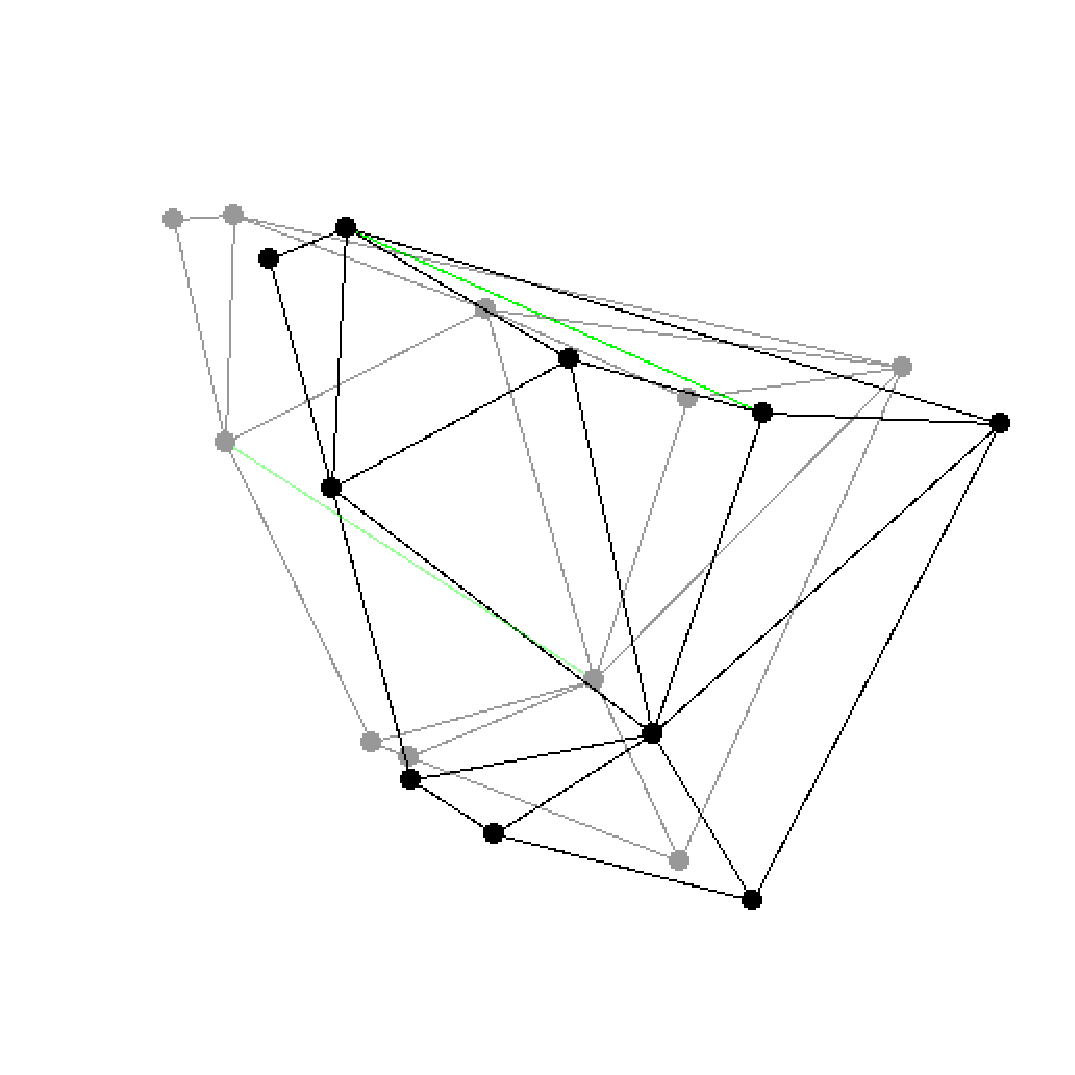
\includegraphics[ scale=.2]{Kinetic_data_structures/delaunay_8}
\end{center}
\end{ccTexOnly}
%width=300 height=300
\begin{ccHtmlOnly}

<img border=1 src="./delaunay_0.gif" align=middle alt="Frame 0" >
<img border=1 src="./delaunay_1.gif" align=middle alt="Frame 1" >
<img border=1 src="./delaunay_2.gif" align=middle alt="Frame 2" >
<img border=1 src="./delaunay_3.gif" align=middle alt="Frame 3" >
<img border=1 src="./delaunay_4.gif" align=middle alt="Frame 4" >
<img border=1 src="./delaunay_5.gif" align=middle alt="Frame 5" >
<img border=1 src="./delaunay_6.gif" align=middle alt="Frame 6" >
<img border=1 src="./delaunay_7.gif" align=middle alt="Frame 7" >
<img border=1 src="./delaunay_8.gif" align=middle alt="Frame 8" >
<br>
\end{ccHtmlOnly}
\caption{ \label{fig:kds_delaunay_events} 
{\em Some events from a Delaunay triangulation kinetic data
structure:} The state of the two dimensional Delaunay triangulation
immediately following the first events is shown. Green edges are ones
which were just created. The pictures are screen shots from
\ccc{demo/Kinetic\_data\_structures/Kinetic\_Delaunay\_triangulation\_2.cpp}. }
%\end{minipage}
%\end{center}
\end{figure*}


\begin{figure}
\begin{ccTexOnly}
\begin{center}
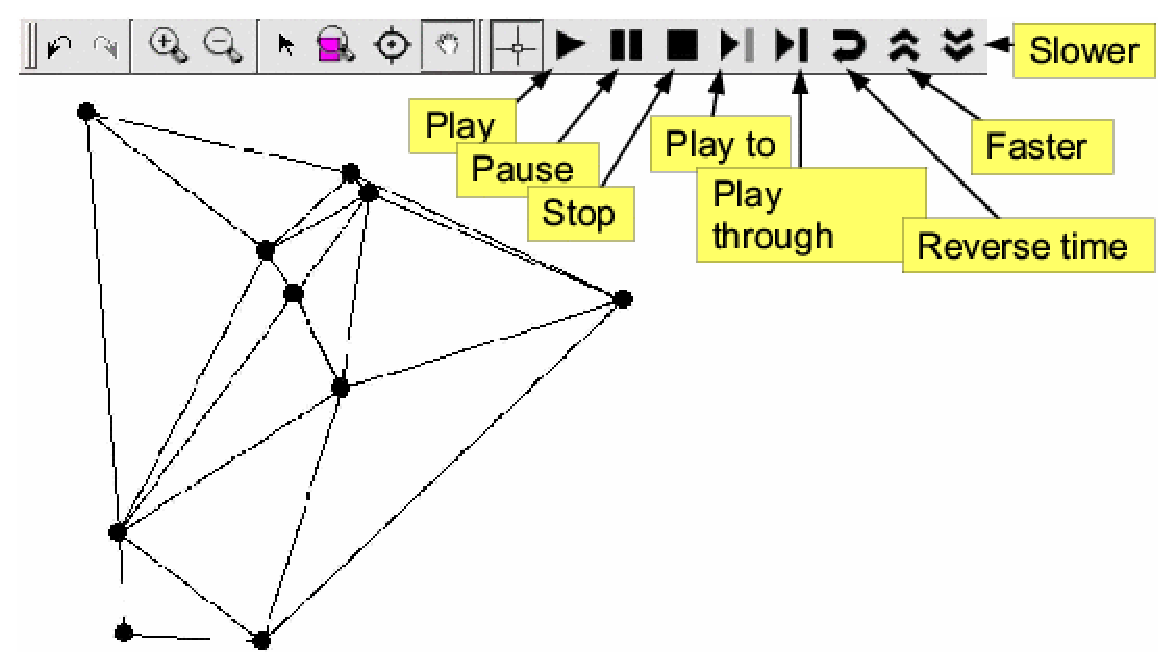
\includegraphics[scale=.5]{Kinetic_data_structures/qt_widget_marked_pct}
\end{center}
\end{ccTexOnly}
\begin{ccHtmlOnly}
<img src="./qt_widget_marked_pct.gif" align=middle alt="Qt widget"> <br>
\end{ccHtmlOnly}
\caption{\label{fig:kds_qtwidget_capture} The figure shows the graphical user interface for
  controlling two-dimensional kinetic data structures. It is built on
  top of the \ccc{Qt_widget} and adds buttons to play, pause, step
  through and run the simulation backwards.}
\end{figure}




\subsection{A Sweepline Algorithm}
\label{sec:sweepline_example}

Here we present a simple example that uses the kinetic data structures
framework to implement a sweepline to compute the arrangement of
x-monotone algebraic curves in the plane. The example builds on top of
the \ccc{Kinetic::Sort<Traits, Visitor>} kinetic data structure, using a visitor
to keep track of changes to the sorted order and newly inserted
points. To see an example using this kinetic data structure read the
example at examples/Kinetic\_data\_structures/sweepline.C.

First we define the visitor class. An object of this type is passed to
the \ccc{Kinetic::Sort} data structure and turns events into calls on
the arrangement structure. This class has to be handled externally
since the arrangement will inherit from the sorting structure.

\begin{ccExampleCode}
template <class Arrangement>
struct Arrangement_visitor: public \ccc{Kinetic::Sort}_visitor_base
{
  Arrangement_visitor(Arrangement *a):p_(a){}
  template <class Vertex_handle>
  void remove_vertex(Vertex_handle a) {
    p_->erase(a);
  }
  template <class Vertex_handle>
  void create_vertex(Vertex_handle a) {
    p_->insert(a);
  }
  template <class Vertex_handle>
  void after_swap(Vertex_handle a, Vertex_handle b) {
    p_->swap(a, b);
  }
  Arrangement *p_;
};

\end{ccExampleCode}

Now we define the actual kinetic data structure. 

\begin{ccExampleCode}

template <class TraitsT> 
class Planar_arrangement: 
  public \ccc{Kinetic::Sort}<TraitsT, 
			     Arrangement_visitor<Planar_arrangement<TraitsT> > > {
  typedef TraitsT Traits;
  typedef Planar_arrangement<TraitsT> This;
  typedef typename \ccc{Kinetic::Sort}<TraitsT,
				       Arrangement_visitor<This> > Sort;
  typedef Arrangement_visitor<This> Visitor;
  typedef typename Traits::Active_objects_table::Key Key;

public:
  typedef CGAL::Exact_predicates_inexact_constructions_kernel::Point_2 Approximate_point;
  typedef std::pair<int,int> Edge;
  typedef typename Sort::Vertex_handle Vertex_handle; 

  // Register this KDS with the MovingObjectTable and the Simulator
  Planar_arrangement(Traits tr): Sort(tr, Visitor(this)) {}

  Approximate_point vertex(int i) const
  {
    return approx_coords_[i];
  }

  size_t vertices_size() const
  {
    return approx_coords_.size();
  }

  typedef std::vector<Edge >::const_iterator Edges_iterator;
  Edges_iterator edges_begin() const
  {
    return edges_.begin();
  }
  Edges_iterator edges_end() const
  {
    return edges_.end();
  }

  void insert(Vertex_handle k) {
    last_points_[*k]=new_point(*k);
  }

  void swap(Vertex_handle a, Vertex_handle b) {
    int swap_point= new_point(*a);
    edges_.push_back(Edge(swap_point, last_points_[*a]));
    edges_.push_back(Edge(swap_point, last_points_[*b]));
    last_points_[*a]= swap_point;
    last_points_[*b]= swap_point;
  }

  void erase(Vertex_handle a) {
    edges_.push_back(Edge(last_points_[*a], new_point(*a)));
  }

  int new_point(typename Traits::Active_objects_table::Key k) {
    double tv= CGAL::to_double(Sort::traits().simulator_handle()->current_time());
    double dv= CGAL::to_double(Sort::traits().active_objects_table_handle()->at(k).x()(tv));
    approx_coords_.push_back(Approximate_point(tv, dv));
    return approx_coords_.size()-1;
  }

  std::vector<Approximate_point > approx_coords_;
  std::map<Key, int> last_points_;
  std::vector<Edge> edges_;

};
\end{ccExampleCode}

%%% Local Variables: 
%%% mode: latex
%%% TeX-master: t
%%% End: 



%%% Local Variables: 
%%% mode: latex
%%% TeX-master: t
%%% End: 



%%%%%%%%%%%%%%%%%%%%%%%%%%%%%%%%%%%%%%%%%%%%%%%%%%%%%%%%%%%%%%%%%%%%
\section{Architecture\label{sec:kds_architecture}}

%%%%%%%%%%%%%%%%%%%%%%%%%%%%%%%%%%%%%%%%%%%%%%%%%%%%%%%%%%%%%%%%%%%%

This package provides a framework to allow exact implementation of
kinetic data structures and sweepline algorithms. Below we discuss in
detail each one of the first four major concepts which help in
implementing kinetic data structures: the \ccc{Kinetic::Simulator},
the \ccc{Kinetic::Kernel}, the \ccc{Kinetic::ActiveObjectsTable} and the
\ccc{Kinetic::InstantaneousKernel}.  The \ccc{Kinetic::FunctionKernel}
concept is discussed separately in Section
\ref{sec:kds_algebraic_kernel}.

\begin{figure}
\begin{ccTexOnly}
\begin{center}
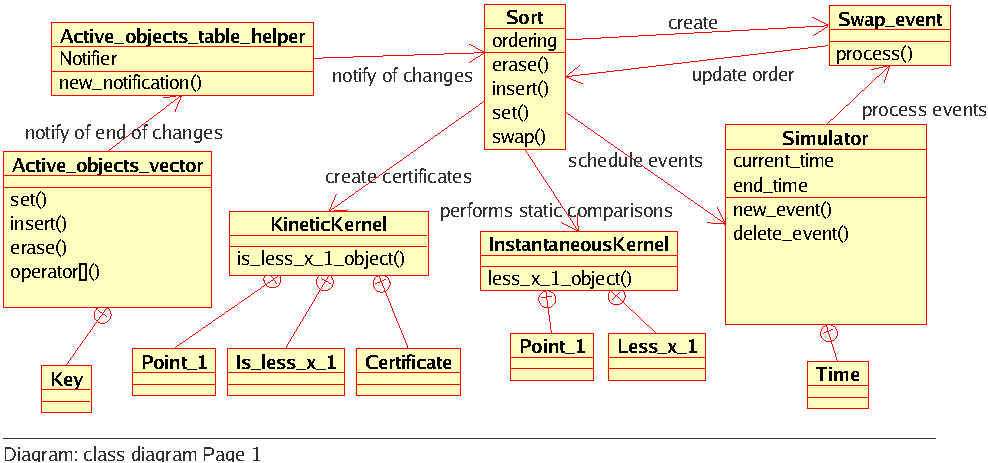
\includegraphics[scale=.8,viewport=0 18 470 250, clip]{Kinetic_data_structures/sort_usage_pct}
\end{center}
\end{ccTexOnly}
\begin{ccHtmlOnly}
<img src="./sort_usage_pct.gif" align=middle alt="Sort Usage"><br>
\end{ccHtmlOnly}
\caption{\label{fig:kds_uml_usage_architecture} The figure, identical
  to the one in the overview of the previous chapter, shows the
  interaction between the \ccc{Kinetic::Sort<Traits, Visitor>} kinetic
  data structure and the various pieces of our framework.  Other, more
  complicated, kinetic data structures will also use the
  \ccc{Kinetic::InstantaneousKernel} in order to insert/remove
  geometric primitives and audit themselves.
  \ccc{Kinetic::Sort<Traits, Visitor>} uses the sorting functionality
  in STL instead.}
\end{figure}

\subsection{The Kinetic::Simulator\label{sec:kds_simulator}}


The \ccc{Kinetic::Simulator} is the central repository of all active events.
It maintains the event queue and can use its knowledge of the events
in the queue to find times for the kinetic data structures to easily
check their own correctness (this will be discussed in more detail
later in this section). Kinetic data structures call methods of the
\ccc{Kinetic::Simulator} to schedule new events, deschedule old ones and
access and change data contained in already scheduled events (the
operations on existing events are performed using a key which was
returned when the event was scheduled).  For controlling the
simulation, methods in the \ccc{Kinetic::Simulator} allow stepping through
events, advancing time and even running the simulation backwards (that
is we run the simulation with the time running in the opposite
direction).

The kinetic sorting example in Figure~\ref{sec:kds_sort_example} shows the
basic usage of the \ccc{Kinetic::Simulator}. First, the \ccc{Simulator}
is created by the \ccc{Kinetic::SimulationTraits}. The kinetic data structure
gets a handle to the simulator from the traits class and uses the
handle to add its events to the simulation. The \ccc{Kinetic::Simulator} is
then told to advance time up until the end of the simulation,
processing all events along the way.

Each event is represented by a \ccc{Kinetic::Simulator::Time} and an instance of a
model of the \ccc{Kinetic::Simulator::Event} concept.  Models of the \ccc{Kinetic::Simulator::Event}
concept are responsible for taking the appropriate action in order to
handle the kinetic event they represent.  Specifically, the
\ccc{Kinetic::Simulator::Event} concept specifies one method,
\ccc{Kinetic::Simulator::Event::process()}, that is called when the event occurs.
The body of the \ccc{Kinetic::Simulator::Event::process()} method typically
simply calls a method of the kinetic data structure that created the
event; for example in our kinetic sorting example, processing an event
means calling the \ccc{Kinetic::Sort<Traits, Visitor>::swap(Iterator)}
method of the kinetic sorting data structure.

In the model of the \ccc{Kinetic::Simulator} concept that we provide,
\ccc{Kinetic:Default_simulator<FunctionKernel, EventQueue>}, any model
of the \ccc{Kinetic::Simulator::Event} concept can be inserted as an
event. This ability implies that events can be mixed at run time,
which is essential when we want to support multiple kinetic data
structures operating on the same set of moving geometric primitives.

The \ccc{Kinetic::Simulator::Time} concept is defined by the simulator, typically to be
some representation of a root of a polynomial, taken from the
\ccc{Kinetic::FunctionKernel} (details of the algebraic side of the package
will be discussed in Section~\ref{sec:kds_algebraic_kernel}). For most
kinetic data structures \ccc{Kinetic::Simulator::Time} only needs to support
comparisons (we need to compare events, in order to process them in
the correct order) and a few other non-arithmetic operations.

When the failure times of certificates are sorted exactly (as opposed
to when we numerically approximate the roots of the certificate
polynomials) the correctness of kinetic data structures can be easily
verified.  Let $I$ be an open interval between the last event
processed and the next event to be processed.  As was mentioned in the
introduction kinetic data structures do not change combinatorially in
$I$. In addition, although the static data structures can be
degenerate at the roots defining the two ends of the interval, they
are not, in general, degenerate in the interior. An independent check
of the integrity of kinetic data structures can be provided by, for
example, using an \ccc{Kinetic::InstantaneousKernel} (cf. Subsection
\ref{sec:kds_instantaneous_kernel}) to rebuild the static version of the
structure from scratch at some time interior to $I$ and compare it to
the kinetic version. This auditing can typically catch algorithmic or
programming errors much closer to the time they arise in the
simulation than, for example, using visual inspection.  Such easy
auditing is one of the powerful advantages of having an exact
computational framework since, as with static data structures, when
using inexact computations differentiating between errors of
implementation and numeric errors is quite tricky.

Kinetic data structures receive alerts of appropriate times to audit
themselves using a notification framework. The same framework is also
used by the \ccc{Kinetic::ActiveObjectsTable} to alert kinetic data
structures when the set of primitives changes (see
Subsection~\ref{sec:kds_active_objects_table}). To use the notification
framework, the kinetic data structure creates a proxy object which
implements a standard \ccc{Listener} interface. It then registers this
proxy with the \ccc{Kinetic::Simulator}. When the
\ccc{Kinetic::Simulator} finds an appropriate time for the kinetic
data structures to audit themselves it calls the function
\ccc{Listener::new_notification(Type)} on each of the registered proxy
objects.  A helper for creating such proxy objects, called
\ccc{Kinetic::Simulator_kds_listener<Listener, KDS>}, is provided by the
framework. It translates the notification into a function call
(\ccc{audit()}) on the kinetic data structure.  Pointers in the
notification framework are reference counted appropriately to avoid
issues caused by the creation and destruction order of kinetic data
structures and the simulator. See Section~\ref{sec:kds_listener} for a more
complete discussion of this part of the framework.

Internally the \ccc{Kinetic::Simulator} maintains a priority queue
containing the scheduled events. The type of the priority queue is a
template argument to our \ccc{Kinetic::Simulator} model and, as such, it can
be replaced by the user.  In our package, we provide two different
types of priority queues, a heap and a two-list priority queue.  A
two-list queue is a queue in which there is a sorted front list,
containing all events before some time and an unsorted back list. The
queue tries to maintain a small number of elements in the front list,
leaving most of them in the unsorted main pool. The two-list queue,
although an unconventional choice, is our default queue when using
exact computation because it minimizes comparisons involving events
that are far in the future.  These events are likely to be deleted
before they are processed, so extra work done structuring them is
wasted.  Our experiments have shown that, for example, the two-list
queue causes a 20\% reduction in running time relative to a binary
heap for Delaunay triangulations with degree 3 polynomial motions and
20 points.



\subsection{The Kinetic::Kernel}

The \ccc{Kinetic::Kernel} is structured very much like static CGAL
kernels. It defines a number of primitives, which in the model
provided are \ccc{Kinetic::Kernel::Point_1},
\ccc{Kinetic::Kernel::Point_2}, \ccc{Kinetic::Kernel::Point_3} and
\ccc{Kinetic::Kernel::Weighted_point_3}. The primitives are defined by
a set of Cartesian coordinates each of which is a function of time, a
\ccc{Kernel::MotionFunction}. In addition it defines constructions
and certificate generators which act on the primitives.  The
certificate generators are the direct analog of the non-kinetic
predicates. Each certificate generator take a number of primitives as
arguments, but instead of producing an element from a discrete set
they produce a set of discrete failure times for the certificate.
These failure times are wrapped in a model of \ccc{Kinetic::Certificate}.

A \ccc{Kinetic::Certificate} is a simple object whose primary function is to
produce a \ccc{Kinetic::Simulator::Time} object representing the failure time of the
certificate.  Since, the handling of most certificate failures
involves creating a new certificate whose certificate function is the
negation of the old certificate function, a \ccc{Kinetic::Certificate}
object caches any work that could be useful to isolate future roots of
the certificate function (such as the Sturm sequence of the
certificate function). To illustrate this further, if you have two
one-dimensional points with coordinate functions $p_0(t)$ and
$p_1(t)$, the certificate that the first moving point is after the
second corresponds to the inequality $p_0(t) - p_1(t) > 0$.  When the
certificate fails and the two points cross, the new certificate is
$p_1(t)- p_0(t) > 0$, which is the negated version of the certificate
just processed and which has the same roots.

The model of \ccc{Kinetic::Kernel} provided includes the certificate
generators necessary for Delaunay triangulations (in one, two and
three dimensions) and regular triangulations (in 3D).  New
certificates can be fairly easily added. An example is included in the
distributed code.



\subsection{The Kinetic::ActiveObjectsTable\label{sec:kds_active_objects_table}}


The \ccc{Kinetic::ActiveObjectsTable} stores a set of kinetic primitives.
Its purpose is to notify kinetic data structures when new primitives
are added, when primitives are removed or when a trajectories change.
Each primitive is uniquely identified by a Key, assigned by
the table when the primitive is added, that can be used to change or
remove it.  We provide one model of the
\ccc{Kinetic::ActiveObjectsTable} concept, called
\ccc{Kinetic::Active_objects_vector<MovingObject>} which stores all the moving
primitives in an \ccc{std::vector<D>}.

Notifications of changes to the set of active objects are handled
using a setup similar to the \ccc{Kinetic::Simulator} audit time
notification. We provide a helper class,
\ccc{Kinetic::Active_objects_listener_helper<ActiveObjectsTable,
KDS>}, which translates the notifications into \ccc{insert(Key)},
\ccc{erase(Key)} or \ccc{set(Key)} function calls on the kinetic data
structure.



\subsection{The Kinetic::InstantaneousKernel\label{sec:kds_instantaneous_kernel}}


The \ccc{Kinetic::InstantaneousKernel} allows existing CGAL data structures
to be used on moving data as it appears at some instant of time.
Models of this concept are, by definition, models of a CGAL
Kernel or a traits class, and, therefore, can then be used as
the traits class of CGAL's algorithms and data structures.

Consider for example the kinetic Delaunay data structure in either two
or three dimensions.  Internally, it uses a
\ccc{Delaunay_triangulation_2<Traits, Tds>} or
\ccc{Delaunay_triangulation_3<Traits, Tds>} to represent the
triangulation, instantiated with a model of the
\ccc{Kinetic::InstantaneousKernel} concept as its traits class.  At
initialization, as well as at times during the simulation when we want
to insert a point to the kinetic Delaunay triangulation, a static
version of the Delaunay triangulation is conceptually instantiated.
More precisely, the time for the copy of the model of the
\ccc{Kinetic::InstantaneousKernel} stored in the CGAL triangulation is set
to be the current time (or rather, as discussed in the introduction, a
more convenient time determined by the \ccc{Kinetic::Simulator}
combinatorially equivalent to the current time).  The kinetic data
structure then calls the
\ccc{Delaunay_triangulation_3<Traits, Tds>::insert(Point)} insert
method to insert the point.  The static insert method called uses
various predicate functors on the moving points which evaluate to the
values that the predicates have at that instant in time. Removal is
handled in an analogous manner. Auditing of the geometric structure is
easily handled in a similar manner (in the case of Delaunay
triangulations by simply calling the \ccc{verify()} method after
setting the time).

%%%%%%%%%%%%%%%%%%%%%%%%%%%%%%%%%%%%%%%%%%%%%%%%%%%%%%%%%%%%%%%%%%%%
\subsection{Miscellaneous: notification and reference management\label{sec:kds_misc}}

%%%%%%%%%%%%%%%%%%%%%%%%%%%%%%%%%%%%%%%%%%%%%%%%%%%%%%%%%%%%%%%%%%%%

We describe some coding conventions used, graphical display,
notification and reference management support in the framework in the
following sections.


\subsubsection{Reference management}

A number of objects need to maintain pointers to other independent
objects. For example, each kinetic data structure must have access to
the \ccc{Kinetic::Simulator} so that it can schedule and deschedule
events. These pointers are all reference counted in order to guarantee
that they are always valid. We provide a standard reference counting
pointer and object base to facilitate this, namely
\ccc{Ref_counted<Object>}.

Each shared object in the framework defines a type \ccc{Handle} which is the
type for a reference counter pointer pointing to it. These should be
used for storing pointers to the objects in order to avoid dangling
pointers. In addition, many of the objects expect such pointers as
arguments.

\subsubsection{Runtime event passing\label{sec:kds_listener}}


Runtime events must be passed from \textit{notifiers}, namely the
\ccc{Kinetic::ActiveObjectsTable} and the \ccc{Kinetic::Simulator} to
\textit{listeners}, typically the kinetic data structures. For
example, kinetic data structures are notified when new primitives are
added to the \ccc{Kinetic::ActiveObjectsTable}. On reciving the
notification, it will add the new primitive to the combinatorial
structure it is maintaining. The events are passed using a simple,
standardized notification interface. To receive notifications, the
listener first defines a small proxy class which inherits from a
\ccc{Listener} base type provided by the notifier. On creation, the
\ccc{Listener} base class registers itself with the notifier on
construction (and unregisters itself on destruction).

When the some state of the notifier changes, it calls the
\ccc{new_notification} method on the listener proxy object provided
and passes it a label corresponding to the name of the field that
changed. The proxy object can then call an appropriate method on the
kinetic data structure or whetever the listening class is.

In order to unregister on destruction, the \ccc{Listener} must store a
(reference counted) pointer to the object providing notifications.
This pointer can be accessed through the \ccc{notifier()} field. The
\ccc{Listener} object stores a reference counted pointer to the
notifying object, while the notifying object stores a plain pointer to
the \ccc{Listener}. It can do this since the \ccc{Listener} is
guaranteed to unregister itself when it is destroyed. This avoids
circular reference counted pointers as well as dangling pointers.

\section{Algebraic Kernel\label{sec:kds_algebraic_kernel}}


The interface between the algebraic kernel and the kinetic data
structures package was kept quite minimal in order to ease the
implementation of various underlying computation models. The interface
is detailed in the reference page (\ccc{Kinetic::FunctionKernel}).

We provide models of the algebraic kernel that handle polynomial
\ccc{Kinetic::Function} objects. The provided models perform
\begin{itemize}
\item exact computations using Sturm sequences to isolate roots
\item exact computations using Descartes rule of sign in order to
  isolate roots (Sturm sequences are also used in order to properly
  handle even multiplicity roots)
\item filtered exact computations using Descartes rule of sign
\item numeric (inexact) root approximations
\item numeric root approximations which take advantage of certain
  assumptions that can be made about the types of polynomials solved
  in the process of evaluating kinetic data structures
\item a wrapper for CORE::Expr which implements the required
  concepts.
\end{itemize}
The exact models, which we implement the numerics for, handle
non-square-free polynomials and polynomials with arbitrary field
number type coefficients and are quite robust.


\subsection{Kinetic::FunctionKernel customized for kinetic data structures}

There are several modifications we can make to how the roots are
handled to optimize for the case of kinetic data structures.  The
first are motivated by the question of how to handle degeneracies
(certificate functions which have roots at the same time).  Naively,
there is no way to differentiate between a certificate which fails
immediately when it is created and one whose function is momentarily
0, but will be valid immediately in the future. In order to handle
such degeneracies we ensure that all the certificate function
generators produce certificate functions which are positive when the
corresponding certificates are valid.  Then, if we have a degeneracy
we can differentiate between a certificate which fails immediately and
one which is simply degenerate by looking at the sign of the
certificate function immediately following the root (equivalently, by
looking at the derivative). In addition, this allows us, under the
assumption that computations are performed exactly, to check that all
certificates are not invalid upon creation.

The assumption that certificates are positive when valid is particular
useful when using numeric solvers.  Without it there is no reliable
way to tell whether a root near the current time is the certificate
having become valid just before the current time, or failing shortly
in the future. Testing the sign of the function immediately after the
root reliably disambiguates the two cases.

In addition, we have to specially handle even roots of functions. For
the most part these can just be discarded as dropping an even root is
equivalent to perturbing the simulation to remove the degeneracy.
However, when we are using the \ccc{Kinetic::Simulator} to audit the
kinetic data structures, they most be broken up in to two, equal,
roots to avoid auditing at the degeneracy.



% Examples
\section{Examples}
\label{AABB_tree_section_examples}

In the following example a set of 3D triangles is stored in a list. The AABB primitive wraps a triangle and an iterator in the list. We computes the number of intersections between a 3D line and the input triangles, and the closest point from a query point to the input triangles.
\ccIncludeExampleCode{AABB_tree/AABB_triangle_3_example.cpp}

The following example computes the number of intersections between a 3D ray and a set of facets of a triangle polyhedral surface. The AABB primitive wraps a facet handle and generates on the fly a 3D triangle each time its object function is called.
\ccIncludeExampleCode{AABB_tree/AABB_polyhedron_facet_example.cpp}

The following example computes the number of intersections between a 3D plane and a set of 3D segments. The segments are stored into a list, and the AABB primitive wraps a segment and an iterator in the list.
\ccIncludeExampleCode{AABB_tree/AABB_segment_3_example.cpp}

The following example computes the number of intersections between a 3D plane and a set of edges of a triangle polyhedral surfaces. The AABB primitive wraps a halfedge handle and generates on the fly a 3D segment each time its object function is called..
\ccIncludeExampleCode{AABB_tree/AABB_polyhedron_edge_example.cpp}




% LocalWords:  Guibas Menelaos CGAL templated Expr KDSs deschedule
% LocalWords:  Karavelas
